\documentclass[a4paper,10pt]{report}
\usepackage[utf8]{inputenc}
\usepackage[francais]{babel}
\usepackage[top=1.5cm, bottom=1.5cm, left=1cm, right=1cm]{geometry}
\usepackage{graphicx}

% Title Page
\title{OMGL4 - Etape 3 : expression des besoins, analyse et conception des autres cas d'utilisation}
\author{MAILLET Arnaud (chef de projet), VARGAS Christophe, ARDAUD Guillaume}


\begin{document}
\maketitle
\newpage
\null
\newpage
\tableofcontents
\newpage
\null
\newpage

\centering

%%%%%%%%%%%%%%%%%%%%%%%%%%%%%%%%%%%%%%%%%%%%%%%%%%%%%%%%%%%%%%%%%%%%%%%%%%%%%%%%%%%%%%%%%%%%%%%%%%%%%%%%%%%%%%%%%%%%%%%%%%%%%%%%%%%%%%%%%%%%%%%%%%%%%%%%%%%%%%%%%%%%%%%%%%%%%%%%%%%%%%%%%%%%%%%%%%%%%%%%%%%%%%%%%%%%%%%%%%%%%%%%%%%%%%%%%%%%%%%%%%%%%%%%%%%%%%%%%%%%%%%%%%%%%%%%%%%%%%%%%%%%%%%%%%%%%%%%%%%%%%%%%%%%%%%%%%

\chapter*{Nouvel ouvrage}
\addcontentsline{toc}{chapter}{Nouvel ouvrage}

Auteur : Christophe VARGAS
Relecteur : Arnaud MAILLET

\bigskip
\section*{Scenario principal}
\addcontentsline{toc}{section}{Scenario principal}
\begin{flushleft}
-
-
-
-
-
\end{flushleft}

\bigskip

\section*{Diagramme de séquence haut niveau}
\addcontentsline{toc}{section}{Diagramme de séquence haut niveau}
% \includegraphics[height=90mm]{}

\newpage

\section*{Unité de présentation}
\addcontentsline{toc}{section}{Unité de présentation}
% \includegraphics[height=70mm]{}

\section*{Diagramme de séquence détaillé MVC}
\addcontentsline{toc}{section}{Diagramme de séquence détaillé MVC}
% \includegraphics[height=150mm]{}

\newpage

%%%%%%%%%%%%%%%%%%%%%%%%%%%%%%%%%%%%%%%%%%%%%%%%%%%%%%%%%%%%%%%%%%%%%%%%%%%%%%%%%%%%%%%%%%%%%%%%%%%%%%%%%%%%%%%%%%%%%%%%%%%%%%%%%%%%%%%%%%%%%%%%%%%%%%%%%%%%%%%%%%%%%%%%%%%%%%%%%%%%%%%%%%%%%%%%%%%%%%%%%%%%%%%%%%%%%%%%%%%%%%%%%%%%%%%%%%%%%%%%%%%%%%%%%%%%%%%%%%%%%%%%%%%%%%%%%%%%%%%%%%%%%%%%%%%%%%%%%%%%%%%%%%%%%%%%%%

\chapter*{Nouveau périodique}
\addcontentsline{toc}{chapter}{Nouveau périodique}

Auteur : Guillaume ARDAUD
Relecteur : Christophe VARGAS

\bigskip
\section*{Scenario principal}
\addcontentsline{toc}{section}{Scenario principal}
\begin{flushleft}
-
-
-
-
-
\end{flushleft}

\bigskip

\section*{Diagramme de séquence haut niveau}
\addcontentsline{toc}{section}{Diagramme de séquence haut niveau}
% \includegraphics[height=90mm]{}

\newpage

\section*{Unité de présentation}
\addcontentsline{toc}{section}{Unité de présentation}
% \includegraphics[height=70mm]{}

\section*{Diagramme de séquence détaillé MVC}
\addcontentsline{toc}{section}{Diagramme de séquence détaillé MVC}
% \includegraphics[height=150mm]{}

\newpage

%%%%%%%%%%%%%%%%%%%%%%%%%%%%%%%%%%%%%%%%%%%%%%%%%%%%%%%%%%%%%%%%%%%%%%%%%%%%%%%%%%%%%%%%%%%%%%%%%%%%%%%%%%%%%%%%%%%%%%%%%%%%%%%%%%%%%%%%%%%%%%%%%%%%%%%%%%%%%%%%%%%%%%%%%%%%%%%%%%%%%%%%%%%%%%%%%%%%%%%%%%%%%%%%%%%%%%%%%%%%%%%%%%%%%%%%%%%%%%%%%%%%%%%%%%%%%%%%%%%%%%%%%%%%%%%%%%%%%%%%%%%%%%%%%%%%%%%%%%%%%%%%%%%%%%%%%%

\chapter*{Nouveau numéro périodique}
\addcontentsline{toc}{chapter}{Nouveau numéro périodique}

Auteur : Arnaud MAILLET
Relecteur : Guillaume ARDAUD

\bigskip

\section*{Scenario principal}
\addcontentsline{toc}{section}{Scenario principal}
\begin{flushleft}
- La documentaliste demande l'enregistrement pour une nouvelle parution d'un périodique donné.\\
- Le système demande le numéro ISSN du périodique.\\
- La documentaliste saisit le numéro ISSN du périodique.\\
- Le système recherche le périodique dans le système informatique et affiche ses informations propres (nom périodique).\\
- Le système demande le numéro de parution de la nouvelle parution.\\
- La documentaliste saisit le numéro de parution de la nouvelle parution\\
- Le système créé la nouvelle parution et lie la nouvelle parution à son periodique.\\
- Le système demande les informations propres des articles de la parution (titre, page).\\
- La documentaliste saisit les informations propres des articles de la parution.\\
- le système crée l'article et lie l'article à la parution du periodique.\\
- Le système demande les auteurs de l'article.\\
- La documentaliste saisit les auteurs de l'article.\\
- Le système recherche les auteurs, les crée si ils n'éxistent pas et les lie à l'article.\\
- Le système demande les mots clés de l'article.\\
- La documentaliste saisit les mots clés de l'article.\\
- Le système recherche les mots clés et les lie à l'article.\\
- Le système confirme l'enregistrement de la nouvelle parution.\\
\end{flushleft}

\bigskip

\section*{Diagramme de séquence haut niveau}
\addcontentsline{toc}{section}{Diagramme de séquence haut niveau}
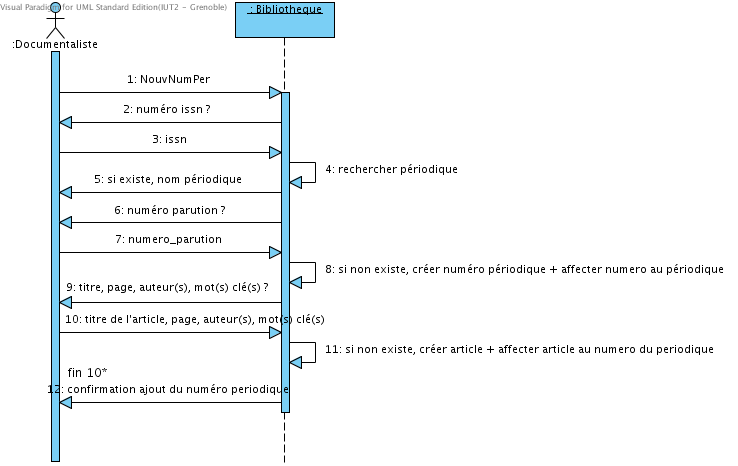
\includegraphics[height=90mm]{NouvNumPerHautNiveau.png}

\newpage

\section*{Unité de présentation}
\addcontentsline{toc}{section}{Unité de présentation}
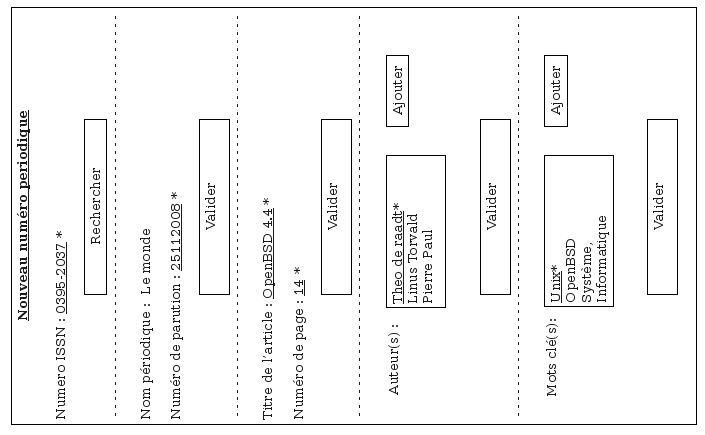
\includegraphics[height=70mm]{UpNouvNumPer.png}

\section*{Diagramme de séquence détaillé MVC}
\addcontentsline{toc}{section}{Diagramme de séquence détaillé MVC}
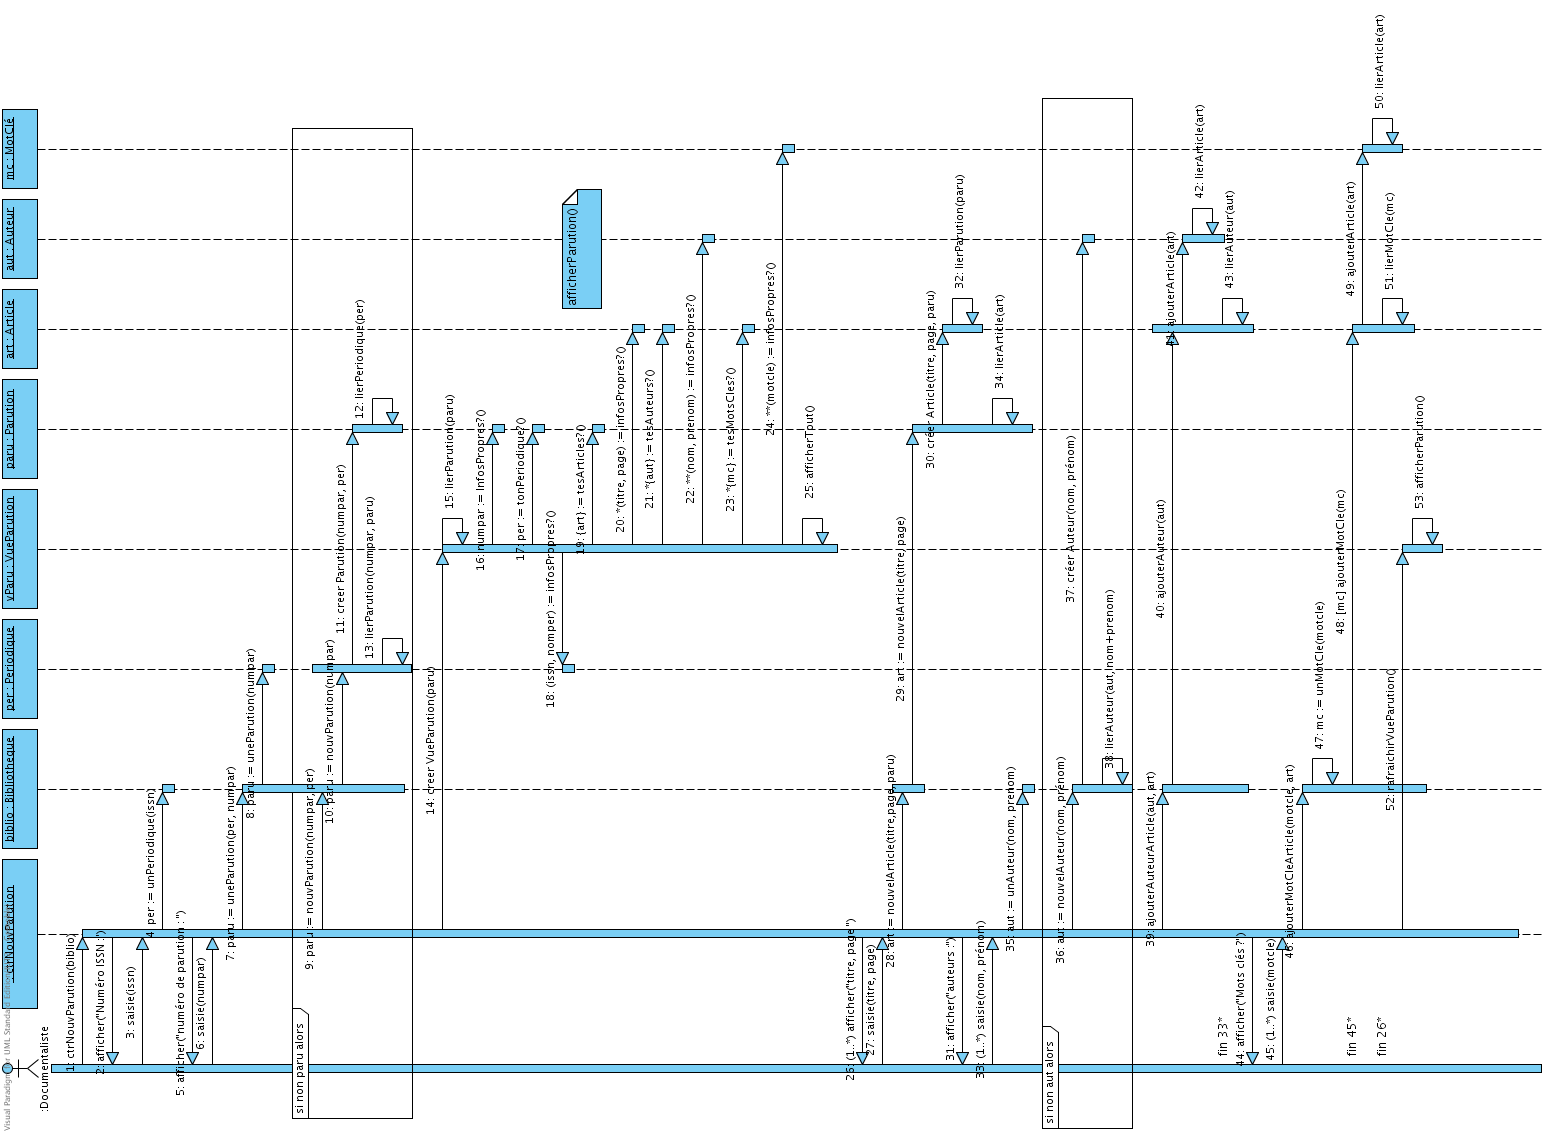
\includegraphics[height=150mm]{NouvNumPerMVC.png}

\newpage

%%%%%%%%%%%%%%%%%%%%%%%%%%%%%%%%%%%%%%%%%%%%%%%%%%%%%%%%%%%%%%%%%%%%%%%%%%%%%%%%%%%%%%%%%%%%%%%%%%%%%%%%%%%%%%%%%%%%%%%%%%%%%%%%%%%%%%%%%%%%%%%%%%%%%%%%%%%%%%%%%%%%%%%%%%%%%%%%%%%%%%%%%%%%%%%%%%%%%%%%%%%%%%%%%%%%%%%%%%%%%%%%%%%%%%%%%%%%%%%%%%%%%%%%%%%%%%%%%%%%%%%%%%%%%%%%%%%%%%%%%%%%%%%%%%%%%%%%%%%%%%%%%%%%%%%%%%

\chapter*{Consulter périodique (avec ses numéros)}
\addcontentsline{toc}{chapter}{Consulter périodique (avec ses numéros)}

Auteur : Christophe VARGAS
Relecteur : Arnaud MAILLET

\bigskip
\section*{Scenario principal}
\addcontentsline{toc}{section}{Scenario principal}
\begin{flushleft}
-
-
-
-
-
\end{flushleft}

\bigskip

\section*{Diagramme de séquence haut niveau}
\addcontentsline{toc}{section}{Diagramme de séquence haut niveau}
%\includegraphics[height=90mm]{}

\newpage

\section*{Unité de présentation}
\addcontentsline{toc}{section}{Unité de présentation}
%\includegraphics[height=70mm]{}

\section*{Diagramme de séquence détaillé MVC}
\addcontentsline{toc}{section}{Diagramme de séquence détaillé MVC}
%\includegraphics[height=150mm]{}

\newpage

%%%%%%%%%%%%%%%%%%%%%%%%%%%%%%%%%%%%%%%%%%%%%%%%%%%%%%%%%%%%%%%%%%%%%%%%%%%%%%%%%%%%%%%%%%%%%%%%%%%%%%%%%%%%%%%%%%%%%%%%%%%%%%%%%%%%%%%%%%%%%%%%%%%%%%%%%%%%%%%%%%%%%%%%%%%%%%%%%%%%%%%%%%%%%%%%%%%%%%%%%%%%%%%%%%%%%%%%%%%%%%%%%%%%%%%%%%%%%%%%%%%%%%%%%%%%%%%%%%%%%%%%%%%%%%%%%%%%%%%%%%%%%%%%%%%%%%%%%%%%%%%%%%%%%%%%%%

\chapter*{Recherche par auteur}
\addcontentsline{toc}{chapter}{Recherche par auteur}

Auteur : Guillaume ARDAUD
Relecteur : Arnaud MAILLET

\bigskip
\section*{Scenario principal}
\addcontentsline{toc}{section}{Scenario principal}
\begin{flushleft}
-
-
-
-
-
\end{flushleft}

\bigskip

\section*{Diagramme de séquence haut niveau}
\addcontentsline{toc}{section}{Diagramme de séquence haut niveau}
%\includegraphics[height=90mm]{}

\newpage

\section*{Unité de présentation}
\addcontentsline{toc}{section}{Unité de présentation}
%\includegraphics[height=70mm]{}

\section*{Diagramme de séquence détaillé MVC}
\addcontentsline{toc}{section}{Diagramme de séquence détaillé MVC}
%\includegraphics[height=150mm]{}

\newpage

%%%%%%%%%%%%%%%%%%%%%%%%%%%%%%%%%%%%%%%%%%%%%%%%%%%%%%%%%%%%%%%%%%%%%%%%%%%%%%%%%%%%%%%%%%%%%%%%%%%%%%%%%%%%%%%%%%%%%%%%%%%%%%%%%%%%%%%%%%%%%%%%%%%%%%%%%%%%%%%%%%%%%%%%%%%%%%%%%%%%%%%%%%%%%%%%%%%%%%%%%%%%%%%%%%%%%%%%%%%%%%%%%%%%%%%%%%%%%%%%%%%%%%%%%%%%%%%%%%%%%%%%%%%%%%%%%%%%%%%%%%%%%%%%%%%%%%%%%%%%%%%%%%%%%%%%%%

\chapter*{Recherche par mot clé}
\addcontentsline{toc}{chapter}{Recherche par mot clé}

Auteur : Arnaud MAILLET
Relecteur : Guillaume ARDAUD

\bigskip
\section*{Scenario principal}
\addcontentsline{toc}{section}{Scenario principal}
\begin{flushleft}
- La documentaliste demande la recherche par mot clé.\\
- Le système demande les mots clés.\\
- La documentaliste saisit les mots clés.\\
- Le système recherche les mots clés et ensuite le système recherche les ouvrages et les articles correspondant à ces mots clés.\\
- Le système affiche la liste des documents.\\
\end{flushleft}

\bigskip

\section*{Diagramme de séquence haut niveau}
\addcontentsline{toc}{section}{Diagramme de séquence haut niveau}
\bigskip
\bigskip
\bigskip
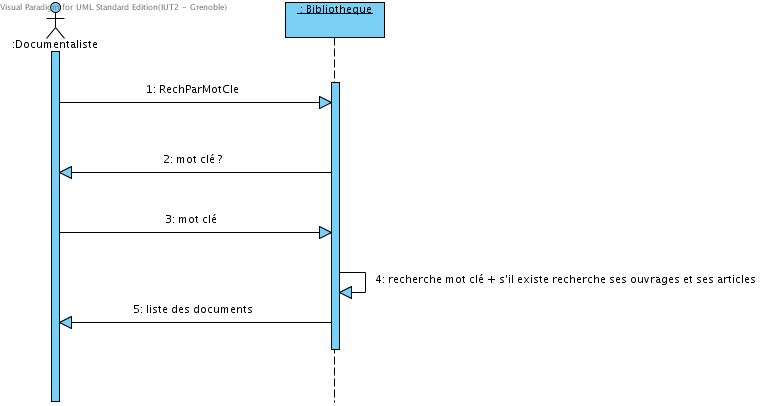
\includegraphics[height=100mm]{RechParMotCleHautNiveau.png}

\newpage

\section*{Unité de présentation}
\addcontentsline{toc}{section}{Unité de présentation}
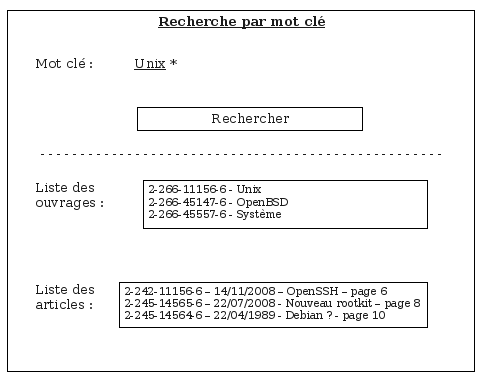
\includegraphics[height=70mm]{UpRechParMotCle.png}

\section*{Diagramme de séquence détaillé MVC}
\addcontentsline{toc}{section}{Diagramme de séquence détaillé MVC}
\bigskip
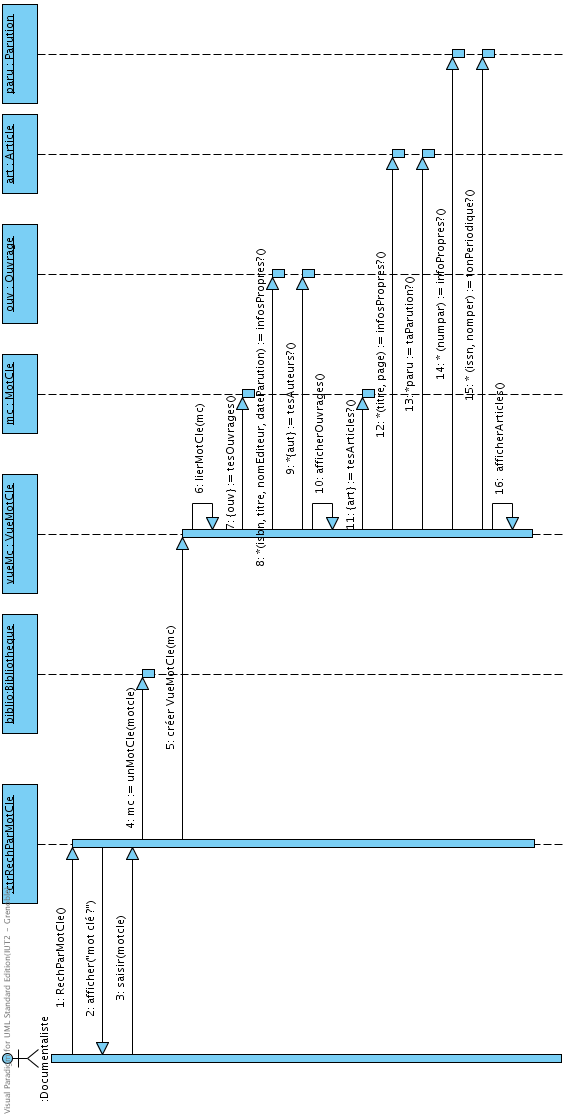
\includegraphics[height=165mm]{RechParMotCleMVC.png}

\newpage

%%%%%%%%%%%%%%%%%%%%%%%%%%%%%%%%%%%%%%%%%%%%%%%%%%%%%%%%%%%%%%%%%%%%%%%%%%%%%%%%%%%%%%%%%%%%%%%%%%%%%%%%%%%%%%%%%%%%%%%%%%%%%%%%%%%%%%%%%%%%%%%%%%%%%%%%%%%%%%%%%%%%%%%%%%%%%%%%%%%%%%%%%%%%%%%%%%%%%%%%%%%%%%%%%%%%%%%%%%%%%%%%%%%%%%%%%%%%%%%%%%%%%%%%%%%%%%%%%%%%%%%%%%%%%%%%%%%%%%%%%%%%%%%%%%%%%%%%%%%%%%%%%%%%%%%%%%

\chapter*{Emprunt exemplaire}
\addcontentsline{toc}{chapter}{Emprunt exemplaire}

Auteur : Guillaume ARDAUD
Relecteur : Christophe VARGAS

\bigskip
\section*{Scenario principal}
\addcontentsline{toc}{section}{Scenario principal}
\begin{flushleft}
-
-
-
-
-
\end{flushleft}

\bigskip

\section*{Diagramme de séquence haut niveau}
\addcontentsline{toc}{section}{Diagramme de séquence haut niveau}
%\includegraphics[height=90mm]{}

\newpage

\section*{Unité de présentation}
\addcontentsline{toc}{section}{Unité de présentation}
%\includegraphics[height=70mm]{}

\section*{Diagramme de séquence détaillé MVC}
\addcontentsline{toc}{section}{Diagramme de séquence détaillé MVC}
%\includegraphics[height=150mm]{}

\newpage

%%%%%%%%%%%%%%%%%%%%%%%%%%%%%%%%%%%%%%%%%%%%%%%%%%%%%%%%%%%%%%%%%%%%%%%%%%%%%%%%%%%%%%%%%%%%%%%%%%%%%%%%%%%%%%%%%%%%%%%%%%%%%%%%%%%%%%%%%%%%%%%%%%%%%%%%%%%%%%%%%%%%%%%%%%%%%%%%%%%%%%%%%%%%%%%%%%%%%%%%%%%%%%%%%%%%%%%%%%%%%%%%%%%%%%%%%%%%%%%%%%%%%%%%%%%%%%%%%%%%%%%%%%%%%%%%%%%%%%%%%%%%%%%%%%%%%%%%%%%%%%%%%%%%%%%%%%

\chapter*{Retour exemplaire}
\addcontentsline{toc}{chapter}{Retour exemplaire}

Auteur : Arnaud MAILLET
Relecteur : Christophe VARGAS

\bigskip
\section*{Scenario principal}
\addcontentsline{toc}{section}{Scenario principal}
\begin{flushleft}
- La documentaliste demande le retour d'un exemplaire.\\
- Le système demande le numéro du lecteur.\\
- La documentaliste saisit le numéro du lecteur.\\
- Le système recherche le lecteur.\\
- Le système demande le numéro ISSN de l'ouvrage et le numéro de l'exemplaire.\\
- La documentaliste saisit le numéro ISSN de l'ouvrage et le numéro de l'exemplaire.\\
- Le système recherche l'exemplaire puis son emprunt, s'ils existent le système enleve le lecteur, l'exemplaire de l'emprunt et détruit l'emprunt.\\
- Le système confirme le retour de l'exemplaire.\\
\end{flushleft}

\bigskip

\section*{Diagramme de séquence haut niveau}
\bigskip
\bigskip
\addcontentsline{toc}{section}{Diagramme de séquence haut niveau}
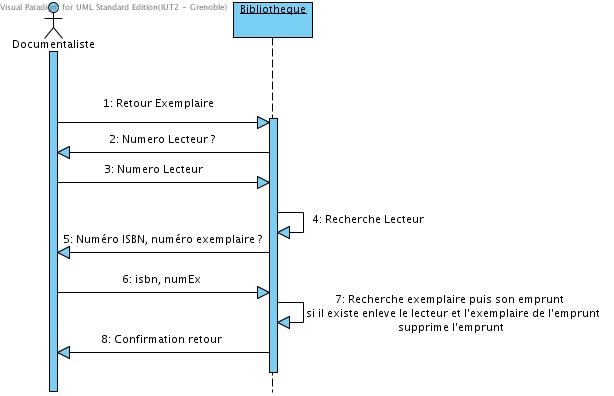
\includegraphics[height=90mm]{RetourExemplaireHautNiveau.png}

\newpage

\section*{Unité de présentation}
\addcontentsline{toc}{section}{Unité de présentation}
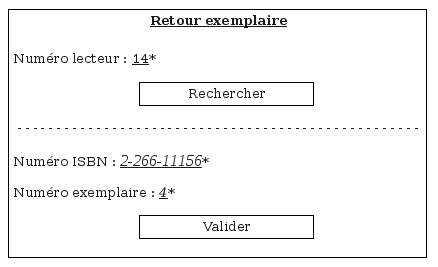
\includegraphics[height=70mm]{UpRetourExemplaire.png}

\section*{Diagramme de séquence détaillé MVC}
\bigskip
\bigskip
\addcontentsline{toc}{section}{Diagramme de séquence détaillé MVC}
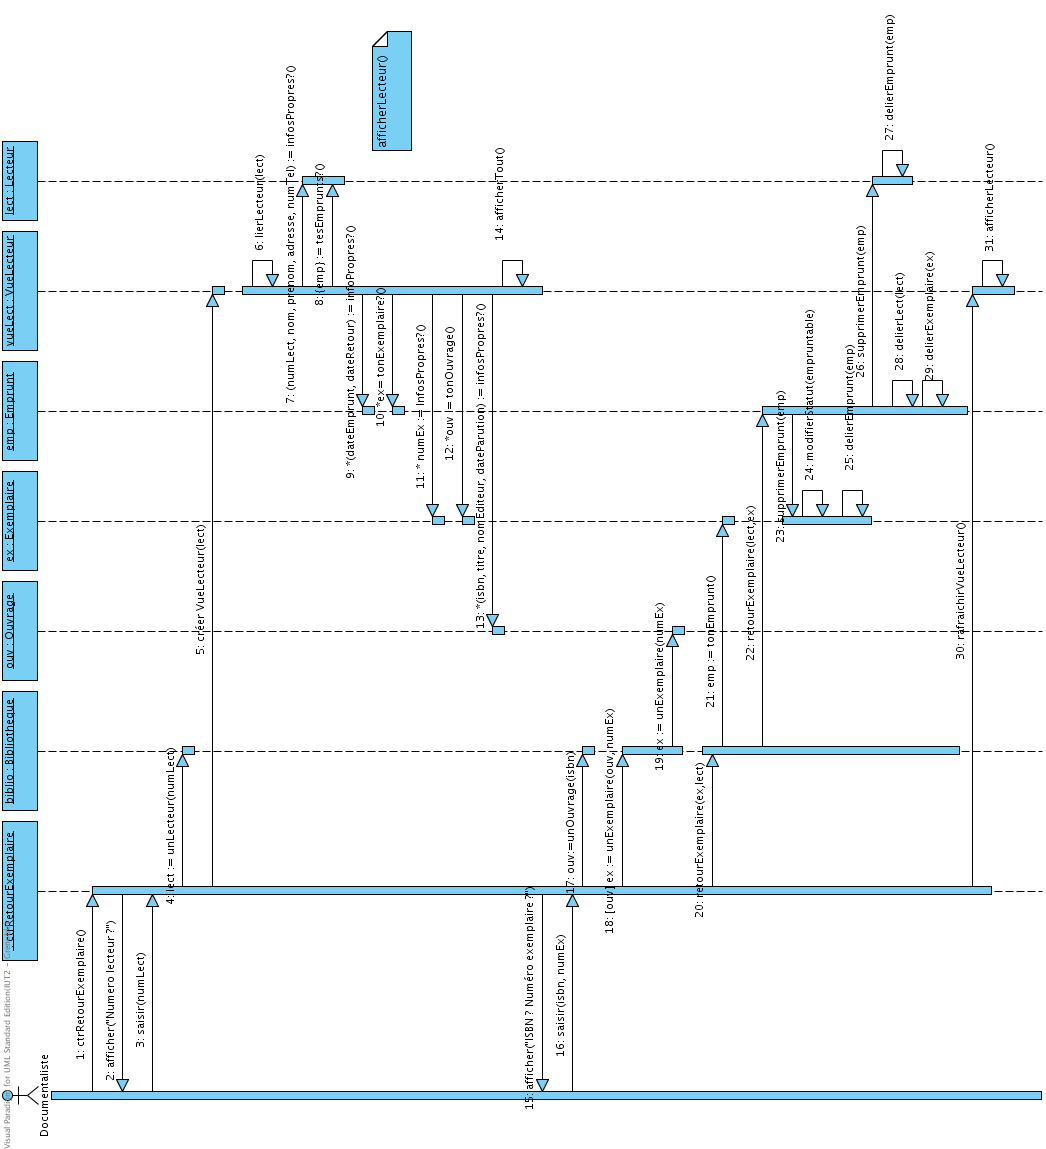
\includegraphics[height=150mm]{RetourExemplaireMVC.png}

\newpage
\end{document}
